\documentclass{article}%
\usepackage[T1]{fontenc}%
\usepackage[utf8]{inputenc}%
\usepackage{lmodern}%
\usepackage{textcomp}%
\usepackage{lastpage}%
\usepackage[head=40pt,margin=0.5in,bottom=0.6in]{geometry}%
\usepackage{graphicx}%
%
\title{\textbf{Habitantes de Bolívar protestaron por no recibir pernil}}%
\author{EL NACIONAL WEB}%
\date{03/12/2018}%
%
\begin{document}%
\normalsize%
\maketitle%
\textbf{URL: }%
http://www.el{-}nacional.com/noticias/protestas/habitantes{-}bolivar{-}protestaron{-}por{-}recibir{-}pernil\_261926\newline%
%
\textbf{Periodico: }%
EN, %
ID: %
261926, %
Seccion: %
Protestas\newline%
%
\textbf{Palabras Claves: }%
Protestas, Sociedad\newline%
%
\textbf{Derecho: }%
2.10%
, Otros Derechos: %
NO\_TIENE%
, Sub Derechos: %
2.10.1%
\newline%
%
\textbf{EP: }%
SI\newline%
\newline%
%
\textbf{\textit{Los manifestantes aseguraron que es el segundo año consecutivo en el que no reciben el alimento}}%
\newline%
\newline%
%
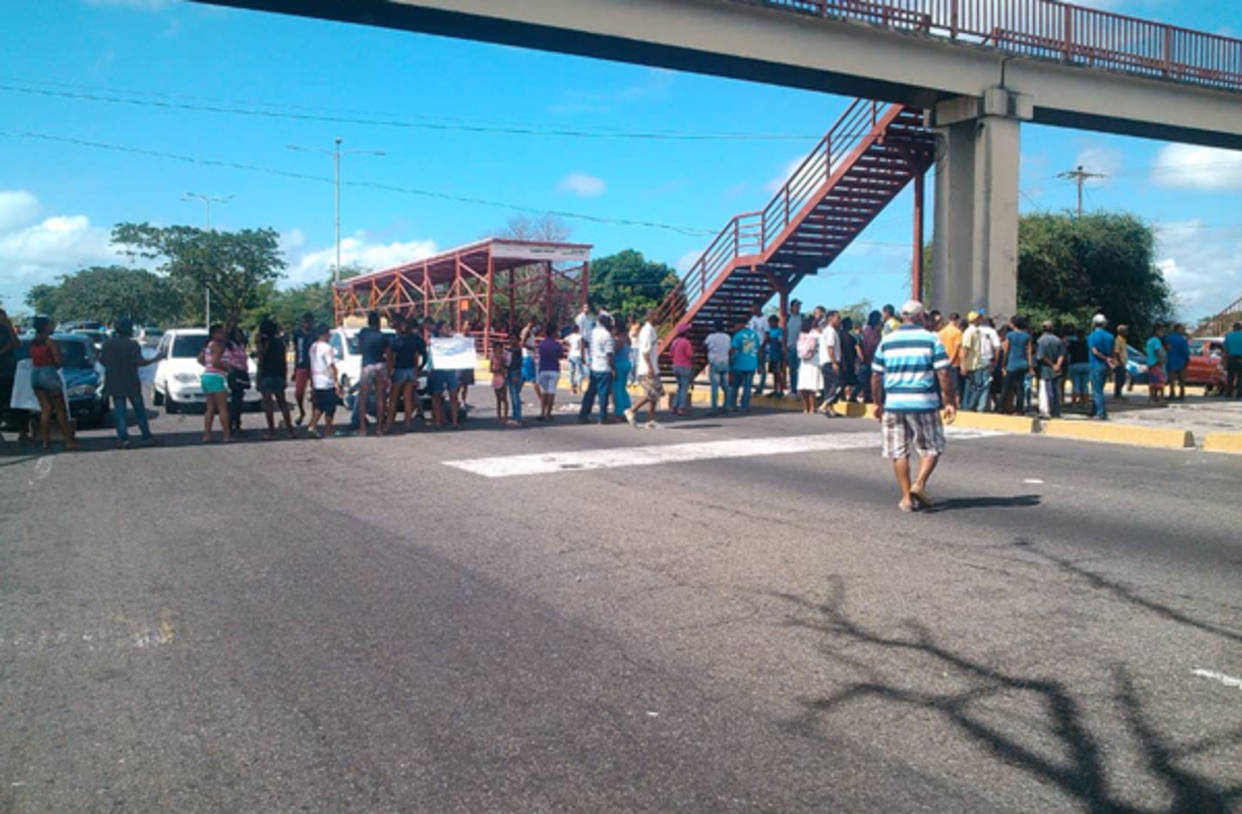
\includegraphics[width=300px]{136.jpg}%
\newline%
%
Habitantes de la parroquia Simón Bolívar, en Ciudad Guayana (estado Bolívar), protestan la mañana de este lunes para reclamar que no han recibido el pernil prometido por el gobierno.%
\newline%
%
La información fue compartida por la periodista Pableysa Ostos, corresponsal de~El Nacional Web, quien informó en su cuenta de Twitter que los ciudadanos cerraron el acceso a la avenida Guayana, a la altura de La Casa de la Mujer.%
\newline%
%
Ostos expresó que los manifestantes aseguraron que es el segundo año consecutivo que no reciben el pernil.%
\newline%
%
\end{document}